\chapter{\IfLanguageName{dutch}{De opstelling en testmethodologie}{The Setup and Testing Methodology}}%
\label{ch:basisopstelling}

\section{Inleiding}

De opstelling is ontworpen met het oog op het evalueren en vergelijken van netwerkprestaties over 4G, publiek 5G en privaat 5G binnen de context van gebouwbeheersystemen, meer bepaald voor toepassingen in verlichting en HVAC-sturing. Aangezien de focus in eerste instantie ligt op netwerkanalyse, wordt gekozen voor een flexibele en programmeerbare testomgeving. In plaats van de oorspronkelijk gekozen Schneider Electric SpaceLogic SmartX AS-P controller wordt een Raspberry Pi gebruikt als centrale testnode.

De Raspberry Pi simuleert de rol van een AS-P controller en voert netwerkmetingen uit, evenals communicatie met gesimuleerde Modbus-apparaten. De meetopstelling is opgebouwd rond een industriële RUTX50-router, die in staat is om zowel 4G als 5G-connectiviteit aan te bieden. Zowel de Raspberry Pi als een Windows-pc zijn bekabeld verbonden met de router voor maximale stabiliteit van de interne netwerkkoppeling.

\section{Motivatie voor gebruik van de Raspberry Pi}

De Raspberry Pi biedt binnen deze meetcontext verscheidene voordelen. Ten eerste biedt het platform een hoge mate van flexibiliteit, aangezien het ondersteuning biedt voor meerdere programmeertalen en bibliotheken, waaronder Python, bash, \texttt{pymodbus}, \texttt{iperf3} en \texttt{speedtest-cli}. Daarnaast maakt de Raspberry Pi een verregaande automatisatie mogelijk, doordat het toelaat complexe testreeksen op een automatische en herhaalbare manier uit te voeren. Tot slot is het toestel bijzonder compact, wat het uitermate geschikt maakt als mobiele meetnode die ingezet kan worden in uiteenlopende netwerkomgevingen.

%TO DO: voorbereiding rasberry pi

\section{Overzicht van de meetopstelling}


% TO DO:Schema maken
\begin{itemize}
    \item De Raspberry Pi en de Windows-pc zijn bekabeld verbonden met een RUTX50-router.
    \item Deze router biedt afwisselend connectiviteit via 4G, publiek 5G en privaat 5G (afhankelijk van de testomgeving).
    \item Op de Raspberry Pi worden diverse scripts uitgevoerd die netwerkparameters meten zoals latency, jitter, throughput, packet loss, en responsiviteit.
    \item De pc fungeert als referentiepunt voor iperf3-sessies en host ook een lokale HTTPS-endpoint via een Python-API.
\end{itemize}

\section{Beschrijving van de uitgevoerde testen}

\subsection{Pingtest (latency en packet loss)}
Om de netwerkprestaties van de Raspberry Pi binnen verschillende netwerkomstandigheden te evalueren, wordt gebruikgemaakt van het \texttt{ping}-commando. Het doel van deze meting is om de gemiddelde latency (rondtriptijd), het aantal verloren pakketten en de spreiding in vertraging (minimum en maximum RTT) tussen de Raspberry Pi en een extern internetadres (in dit geval het publieke DNS-adres van Google, 8.8.8.8) in kaart te brengen.

Het gebruikte commando is als volgt: \textbf{ping -c 250 8.8.8.8 > ping*.log}

In dit commando staat \texttt{'-c 250'} voor het aantal echo-verzoeken dat naar het opgegeven IP-adres wordt gestuurd, in dit geval worden er dus 250 ICMP-pakketten verzonden. De output van het commando wordt omgeleid naar een logbestand met de naam \texttt{ping*.log}, waarin \texttt{*} verwijst naar een unieke identificatie per testreeks (bijvoorbeeld: ping4g1.log).

De metingen worden vier keer uitgevoerd per netwerkmodus zowel voor 4G als voor 5G waardoor er per technologie in totaal 1000 individuele metingen beschikbaar zijn. Deze opzet maakt het mogelijk om statistisch relevante conclusies te trekken over de prestaties van elk netwerk.

De belangrijkste doelvariabelen die uit deze metingen worden afgeleid, zijn de gemiddelde latency, het minimum en maximum van de round-trip time (RTT), en het percentage pakketverlies. Deze grootheden geven samen een goed beeld van de stabiliteit en efficiëntie van de netwerkverbinding onder verschillende omstandigheden.

\subsection{TCP throughputtest (bandbreedte en betrouwbaarheid)}
In deze meting wordt de nadruk gelegd op het bepalen van de netto datadoorvoer en de stabiliteit van de TCP-verbinding tussen de Raspberry Pi en een externe pc. De metingen worden uitgevoerd met behulp van de tool \texttt{iperf3}, die specifiek ontworpen is voor performantie-evaluaties van netwerkverbindingen.

De testopstelling vereist dat de iperf3-server op de ontvangende pc wordt geactiveerd. Download iperf3 voor Windows via: 'https://iperf.fr/iperf-download.php'. De server wordt dan gestart via het volgende commando: \textbf{iperf3.exe -s} 

Zodra de server actief is, wordt de Raspberry Pi geconfigureerd als client en voert deze het volgende commando uit: \textbf{iperf3 -c [PC-IP] -t 120 > iperf*.log}

In dit commando vervangt \texttt{[PC-IP]} het IP-adres van de pc waarop de server draait. De vlag \texttt{-t 120} specificeert dat de meting gedurende 120 seconden (twee minuten) wordt uitgevoerd. De uitvoer wordt opgeslagen in een logbestand met een herkenbare naam (\texttt{iperf*.log}), waarbij \texttt{*} verwijst naar de specifieke testomstandigheden.

Voor elke netwerkomgeving 4G en 5G worden vier aparte sessies uitgevoerd, telkens met een duur van twee minuten. Dit zorgt voor een voldoende representatieve steekproef om statistische vergelijkingen mogelijk te maken.

De analyse van de resultaten richt zich op de doorvoersnelheid per seconde, de variatie in die snelheden over de volledige sessie (als maat voor stabiliteit), en het aantal eventuele TCP-retransmissies, wat een indicatie geeft van netwerkbetrouwbaarheid en congestie. Deze parameters bieden samen een diepgaand inzicht in de prestaties van het TCP-protocol onder reële omstandigheden.


\subsection{HTTP latency test (toepassingslatency)}
Het doel van deze meting is het simuleren van een realistische netwerkinteractie met een webgebaseerde API, zoals die typisch gebruikt wordt in smart building dashboards of Internet of Things (IoT)-toepassingen. Dit laat toe om niet enkel de ruwe netwerkprestaties, maar ook de gebruikerservaring bij API-interacties te evalueren.

Voor de test wordt op de pc een lokale webserver opgezet met behulp van een python script 'api.py' en is bereikbaar via het interne IP-adres van de pc. 

%TO DO: listings bekijken
%\begin{Verbatim}
%    from http.server import BaseHTTPRequestHandler, HTTPServer
%    import json
%    
%    class SimpleHandler(BaseHTTPRequestHandler):
%    def do_POST(self):
%    content_length = int(self.headers['Content-Length'])
%    post_data = self.rfile.read(content_length)
%    print("Ontvangen data:", post_data.decode('utf-8'))
%    
%    self.send_response(200)
%    self.send_header('Content-type', 'application/json')
%    self.end_headers()
%    response = {'status': 'OK'}
%    self.wfile.write(json.dumps(response).encode('utf-8'))
%    
%    server = HTTPServer(('0.0.0.0', 8080), SimpleHandler)
%    print("Mock API draait op http://localhost:8080")
%    server.serve_forever()
%\end{Verbatim}

Op de Raspberry Pi wordt een shellscript genaamd \texttt{gbssim.sh} uitgevoerd. Dit script stuurt in totaal 250 HTTP GET-verzoeken naar de API-endpoint via een For-lus en meet per verzoek meerdere tijdsparameters met behulp van het time curl-commando. Het commando: \textbf{time curl -k -X POST http://[endpoint] -d '\{"status": "ok"\}' -H "Content-Type: application/json"}

Het script maakt gebruik van de \texttt{curl}-tool, waarbij elke aanvraag wordt geanalyseerd op drie kernparameters: de time to connect (tijd tot succesvolle TCP-handshake), de time to first byte (vertraging tot de server begint te antwoorden), en de totale responstijd. Deze gegevens bieden waardevolle inzichten in zowel de netwerklaag als de prestaties van de API zelf.

De test wordt vier keer herhaald per netwerkmodus, wat resulteert in 1000 individuele HTTP-verzoeken per technologie. Dankzij deze herhaling kan men de stabiliteit van de netwerkinteractie beoordelen en eventuele fluctuaties of latentiepieken identificeren.

De verzamelde gegevens worden geanalyseerd met het oog op consistentie, betrouwbaarheid van de verbinding en gebruikservaring, wat essentieel is voor toepassingen in real-time monitoring en besturingssystemen binnen slimme gebouwen.


\subsection{UDP jittertest}
Om de eigenschappen van een niet-verbindingsgerichte netwerkoverdracht te analyseren, wordt een meting uitgevoerd met het UDP-protocol. In tegenstelling tot TCP, biedt UDP geen garantie op levering of volgorde, waardoor deze test specifiek gericht is op het bepalen van jitter (variatie in vertraging tussen opeenvolgende pakketten) en het aantal verloren pakketten. Beide zijn cruciale parameters voor real-time toepassingen zoals VoIP of videostreaming.

De meting wordt uitgevoerd met behulp van \texttt{iperf3}, waarbij de Raspberry Pi als client fungeert en een pc met actieve \texttt{iperf3}-server als ontvanger. Het volgende commando wordt op de Raspberry Pi gebruikt: \textbf{iperf3 -c [PC-IP] -u -b xM -t 120 > iperfudp*.log}

In dit commando specificeert de vlag \texttt{-u} dat het om een UDP-verbinding gaat. Met \texttt{-b xM} wordt de bandbreedte vastgelegd op x megabit(s) per seconde. De testduur wordt ingesteld op 120 seconden via \texttt{-t 120}, en de uitvoer wordt gelogd in een bestand genaamd \texttt{iperfudp*.log}, waarbij \texttt{*} een placeholder is voor de testconfiguratie of het sessienummer. Het IP-adres van de pc-server moet worden ingevuld op de plaats van \texttt{[PC-IP]}.

De test wordt viermaal herhaald per netwerkomgeving en met de waardes x = (1,5,50) wat een robuuste dataset oplevert om verschillen tussen technologieën te kunnen detecteren. 

Tijdens de analyse worden drie hoofdparameters geëvalueerd: de jitter, het absolute aantal verloren pakketten, en de verhouding van verloren tot totaal verzonden pakketten (Lost/Total ratio). Deze meetwaarden bieden een nauwkeurig inzicht in de betrouwbaarheid en stabiliteit van de UDP-verbinding, en zijn van bijzonder belang bij het beoordelen van de geschiktheid van een netwerk voor latency-gevoelige toepassingen.


\subsection{Speedtest via Node-RED}
In deze testopstelling wordt gebruikgemaakt van Node-RED, een visueel programmeerplatform dat vaak wordt ingezet binnen IoT-toepassingen voor het beheren van datastromen tussen sensoren, servers en applicaties. Het doel van deze meting is het evalueren van de download- en uploadsnelheden binnen een realistische en visuele omgeving, die representatief is voor veelgebruikte IoT-dashboards.

% verwijzing naar server.js
Node-RED wordt lokaal opgestart op de Raspberry Pi met het commando \textbf{node-red}. De gebruikersinterface van Node-RED is toegankelijk via het interne IP-adres van de Pi op poort 1880, bijvoorbeeld via: 'http://[IP-Pi]:1880'

%TO DO: foto flow + uitleg

De gebruikte flow, weergegeven in Figuur~\ref{fig:nodered-flow}, bestaat uit drie knooppunten: een \texttt{inject}-node (timestamp), een \texttt{exec}-node met een \texttt{curl}-commando, en een \texttt{debug}-node. Bij activatie verstuurt het systeem via \texttt{curl} een HTTP POST-verzoek naar een endpoint op een externe pc: \textbf{curl -k -X POST http://192.168.1.40:8080 -d '{"value":42}' -H "Content-Type: application/json"}

Hierbij staat \texttt{-k} toe dat een onveilige (zelfondertekende) verbinding wordt geaccepteerd, \texttt{-X POST} specificeert het HTTP-methodetype, en de data wordt in JSON-formaat verstuurd met de correcte content header. Deze opzet bootst realistische API-interacties na, zoals ze vaak voorkomen in IoT-systemen waarbij sensorgegevens of statussen naar een centrale dienst worden gepusht.

De test wordt gedurende ongeveer zeven minuten uitgevoerd, wat voldoende is om een representatief aantal metingen te verzamelen. De nadruk ligt op het analyseren van drie hoofdparameters: de variabiliteit van de overdrachtssnelheden, de maximale piekwaarden en de gemiddelde snelheid tijdens de testperiode. 

\begin{figure}[h]
    \centering
    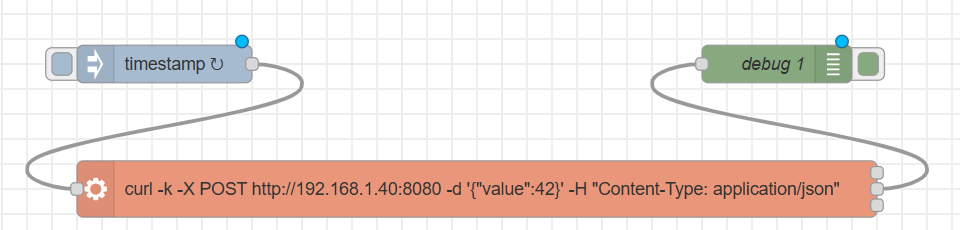
\includegraphics[width=0.9\textwidth]{../graphics/node-red_flow.png}
    \caption{Node-RED-flow voor het verzenden van HTTP POST-verzoeken naar een externe endpoint.}
    \label{fig:nodered-flow}
\end{figure}

Deze aanpak combineert een visuele programmeerstijl met krachtige shellcommando’s, wat bijzonder nuttig is in edge computing-toepassingen waar lichtgewicht IoT-devices lokaal data moeten verwerken of doorsturen. De flexibiliteit en transparantie van de metingen maken deze methode geschikt voor zowel prestatieanalyse als validatie in testomgevingen.


\subsection{Smart verlichting test}
Het doel van deze meting is het evalueren van de betrouwbaarheid en de reactietijd van een eenvoudige IoT-toepassing in functie van de onderliggende netwerkverbinding. Hierbij wordt specifiek onderzocht in welke mate de netwerktechnologie (4G versus 5G) een invloed heeft op de snelheid en betrouwbaarheid waarmee een commando van een client naar een slim toestel wordt uitgevoerd.

Voor deze testopstelling wordt geen gebruik gemaakt van de Raspberry Pi. In plaats daarvan staat een Philips Hue Bridge centraal, die verbonden is met het netwerk via een bekabelde ethernetverbinding. De slimme lamp die via deze bridge wordt aangestuurd, fungeert als uitvoerend toestel. 

Het centrale testscript, \texttt{lichtscript.py}, is geschreven in Python en maakt gebruik van de Hue API. Het script voert bij elke iteratie twee opeenvolgende toggle-operaties uit (aan-uit of uit-aan) op de lamp. Elke uitvoering wordt gelogd, inclusief de timestamp van het verzonden commando en de timestamp waarop de actie visueel bevestigd werd (via logging of sensorfeedback).

%\begin{Verbatim}{python}
%    import requests
%    import time
%    import csv
%    from datetime import datetime
%    
%    BRIDGE_IP = "10.5.0.185"
%    USERNAME = "drs7MVr-eK2e4HiBlzXMbsWCAPIiD24rMjHwKcx3"
%    LIGHT_ID = "1"
%    URL = f"http://{BRIDGE_IP}/api/{USERNAME}/lights/{LIGHT_ID}/state"
%    AANTAL_TESTS = 200
%    CSV_BESTAND = f"betrouwbaarheid_test_{datetime.now().strftime('%Y%m%d_%H%M%S')}.csv"
%    
%    def toggle_light(state):
%    payload = {"on": state}
%    start = time.time()
%    try:
%    response = requests.put(URL, json=payload, timeout=5)
%    end = time.time()
%    duur = round((end - start)*1000, 2)  # in ms
%    
%    if response.status_code == 200:
%    return True, duur, response.json()
%    else:
%    return False, duur, response.text
%    except Exception as e:
%    return False, None, str(e)
%    
%    # === TESTLOOP ===
%    resultaten = []
%    print(f"Start betrouwbaarheidstest ({AANTAL_TESTS} commando’s)...")
%    
%    for i in range(AANTAL_TESTS):
%    state = i % 2 == 0  # om en om: aan/uit
%    success, duur, reactie = toggle_light(state)
%    
%    resultaten.append({
%        "nummer": i + 1,
%        "actie": "aan" if state else "uit",
%        "resultaat": "succes" if success else "fout",
%        "reactietijd_ms": duur if duur else "n.v.t.",
%        "response": reactie
%    })
%    
%    status = "true" if success else "false"
%    print(f"[{i+1:03}] {status} - {'aan' if state else 'uit'} - {duur if duur else 'n.v.t.'} ms")
%    
%    time.sleep(1)  # optioneel vertraging tussen commando’s
%    
%    # === RESULTATEN SCHRIJVEN NAAR CSV ===
%    with open(CSV_BESTAND, mode='w', newline='', encoding='utf-8') as f:
%    writer = csv.DictWriter(f, fieldnames=resultaten[0].keys())
%    writer.writeheader()
%    writer.writerows(resultaten)
%    
%    # === OVERZICHT TONEN ===
%    aantal_succes = sum(1 for r in resultaten if r["resultaat"] == "succes")
%    aantal_fout = AANTAL_TESTS - aantal_succes
%    gemiddelde_tijd = round(sum(r["reactietijd_ms"] for r in resultaten if isinstance(r["reactietijd_ms"], float)) / aantal_succes, 2)
%    
%    print("\nRESULTAATOVERZICHT")
%    print(f"Succesvolle commando's : {aantal_succes}")
%    print(f"Mislukte commando's     : {aantal_fout}")
%    print(f"Gemiddelde reactietijd : {gemiddelde_tijd} ms")
%    print(f"CSV opgeslagen als: {CSV_BESTAND}")
%\end{Verbatim}

%TO DO: uitleggen script

De kernparameter die gemeten wordt, is de totale tijd tussen het initiëren van het commando en het effectief voltooien van de toggle-operatie. Eventuele fouten (bv. timeouts of mislukte requests) worden eveneens geregistreerd als indicatoren voor netwerkbetrouwbaarheid.

De test wordt uitgevoerd in twee netwerkmodi: via een 4G-verbinding en via een 5G-verbinding. Per modus worden 100 iteraties uitgevoerd van het script, met telkens twee toggles per iteratie. Dit resulteert in 200 metingen per technologie en 400 metingen in totaal.

Deze experimentele opzet laat toe om te evalueren hoe netwerkvertragingen en -stabiliteit impact hebben op de werking van een eenvoudige maar representatieve IoT-schakeling. De resultaten leveren waardevolle inzichten op voor het gebruik van mobiele netwerken in real-time of near-real-time besturingssystemen binnen smart home- of smart building-contexten.


\section{Samenvatting van meetdoelen}

%TO DO: nog eens bekijken

Het volledige testkader is ontworpen om gericht antwoord te bieden op drie centrale onderzoeksvragen met betrekking tot de performantie van mobiele netwerken in een smart building-context. Elke afzonderlijke test draagt bij tot het genereren van zowel kwantitatieve meetgegevens als kwalitatieve inzichten, met als doel een diepgaand vergelijkend beeld te verkrijgen tussen verschillende netwerktechnologieën.

De eerste onderzoeksvraag richt zich op het objectief vergelijken van netwerkparameters: \textit{Wat is het verschil in latency, jitter, packet loss en throughput tussen 4G, publiek 5G en privaat 5G?} Via geautomatiseerde metingen, waaronder \texttt{ping}, \texttt{iperf3} en \texttt{speedtest-cli}, worden deze prestatieparameters systematisch vastgelegd in gecontroleerde testomstandigheden. De analyse hiervan verschaft inzicht in de fundamentele technische eigenschappen van elk netwerktype.

Een tweede onderzoeksvraag heeft betrekking op de betrouwbaarheid van netwerkcommunicatie in functionele toepassingen: \textit{Hoe betrouwbaar verlopen netwerkverzoeken en IoT-acties in een smart building scenario over verschillende mobiele netwerken?} Deze vraag wordt beantwoord aan de hand van simulaties van realistische applicaties, zoals het opvragen van data via HTTP, het schakelen van slimme verlichting en het communiceren met webgebaseerde dashboards via Node-RED. Daarbij wordt zowel het succespercentage als de reactietijd van de interacties gemeten.

De derde onderzoeksvraag onderzoekt de bredere impact van netwerkprestaties op systeemniveau: \textit{In welke mate beïnvloeden de netwerkparameters de performantie van gebouwbeheersystemen?} Door de netwerkmetingen te koppelen aan specifieke applicatieresultaten — bijvoorbeeld de responstijd van een sensorupdate of de betrouwbaarheid van een besturingssignaal — kan worden geëvalueerd hoe gevoelig dergelijke systemen zijn voor vertragingen, packet loss of fluctuaties in bandbreedte.

Deze multidimensionale teststructuur biedt aldus een gebalanceerd perspectief waarin zowel lage-level netwerkstatistieken als high-level functionele performantie geïntegreerd geanalyseerd worden. Dit maakt het mogelijk om gefundeerde uitspraken te doen over de geschiktheid van verschillende mobiele netwerken voor kritieke IoT-toepassingen binnen slimme gebouwen en andere latency-gevoelige omgevingen.

